\documentclass[man]{apa6}
\usepackage{lmodern}
\usepackage{amssymb,amsmath}
\usepackage{ifxetex,ifluatex}
\usepackage{fixltx2e} % provides \textsubscript
\ifnum 0\ifxetex 1\fi\ifluatex 1\fi=0 % if pdftex
  \usepackage[T1]{fontenc}
  \usepackage[utf8]{inputenc}
\else % if luatex or xelatex
  \ifxetex
    \usepackage{mathspec}
  \else
    \usepackage{fontspec}
  \fi
  \defaultfontfeatures{Ligatures=TeX,Scale=MatchLowercase}
\fi
% use upquote if available, for straight quotes in verbatim environments
\IfFileExists{upquote.sty}{\usepackage{upquote}}{}
% use microtype if available
\IfFileExists{microtype.sty}{%
\usepackage{microtype}
\UseMicrotypeSet[protrusion]{basicmath} % disable protrusion for tt fonts
}{}
\usepackage{hyperref}
\hypersetup{unicode=true,
            pdftitle={Personality and political beliefs across the lifespan},
            pdfauthor={Sarah Dimakis, Meghan Siritzky, \& Jamie Yellowtail},
            pdfkeywords={keywords},
            pdfborder={0 0 0},
            breaklinks=true}
\urlstyle{same}  % don't use monospace font for urls
\usepackage{graphicx,grffile}
\makeatletter
\def\maxwidth{\ifdim\Gin@nat@width>\linewidth\linewidth\else\Gin@nat@width\fi}
\def\maxheight{\ifdim\Gin@nat@height>\textheight\textheight\else\Gin@nat@height\fi}
\makeatother
% Scale images if necessary, so that they will not overflow the page
% margins by default, and it is still possible to overwrite the defaults
% using explicit options in \includegraphics[width, height, ...]{}
\setkeys{Gin}{width=\maxwidth,height=\maxheight,keepaspectratio}
\IfFileExists{parskip.sty}{%
\usepackage{parskip}
}{% else
\setlength{\parindent}{0pt}
\setlength{\parskip}{6pt plus 2pt minus 1pt}
}
\setlength{\emergencystretch}{3em}  % prevent overfull lines
\providecommand{\tightlist}{%
  \setlength{\itemsep}{0pt}\setlength{\parskip}{0pt}}
\setcounter{secnumdepth}{0}
% Redefines (sub)paragraphs to behave more like sections
\ifx\paragraph\undefined\else
\let\oldparagraph\paragraph
\renewcommand{\paragraph}[1]{\oldparagraph{#1}\mbox{}}
\fi
\ifx\subparagraph\undefined\else
\let\oldsubparagraph\subparagraph
\renewcommand{\subparagraph}[1]{\oldsubparagraph{#1}\mbox{}}
\fi

%%% Use protect on footnotes to avoid problems with footnotes in titles
\let\rmarkdownfootnote\footnote%
\def\footnote{\protect\rmarkdownfootnote}


  \title{Personality and political beliefs across the lifespan}
    \author{Sarah Dimakis\textsuperscript{1}, Meghan Siritzky\textsuperscript{1}, \&
Jamie Yellowtail\textsuperscript{1}}
    \date{}
  
\shorttitle{PERSONALITY AND POLITICAL BELIEFS}
\affiliation{
\vspace{0.5cm}
\textsuperscript{1} University of Oregon}
\keywords{keywords\newline\indent Word count: X}
\usepackage{csquotes}
\usepackage{upgreek}
\captionsetup{font=singlespacing,justification=justified}

\usepackage{longtable}
\usepackage{lscape}
\usepackage{multirow}
\usepackage{tabularx}
\usepackage[flushleft]{threeparttable}
\usepackage{threeparttablex}

\newenvironment{lltable}{\begin{landscape}\begin{center}\begin{ThreePartTable}}{\end{ThreePartTable}\end{center}\end{landscape}}

\makeatletter
\newcommand\LastLTentrywidth{1em}
\newlength\longtablewidth
\setlength{\longtablewidth}{1in}
\newcommand{\getlongtablewidth}{\begingroup \ifcsname LT@\roman{LT@tables}\endcsname \global\longtablewidth=0pt \renewcommand{\LT@entry}[2]{\global\advance\longtablewidth by ##2\relax\gdef\LastLTentrywidth{##2}}\@nameuse{LT@\roman{LT@tables}} \fi \endgroup}


\DeclareDelayedFloatFlavor{ThreePartTable}{table}
\DeclareDelayedFloatFlavor{lltable}{table}
\DeclareDelayedFloatFlavor*{longtable}{table}
\makeatletter
\renewcommand{\efloat@iwrite}[1]{\immediate\expandafter\protected@write\csname efloat@post#1\endcsname{}}
\makeatother
\usepackage{lineno}

\linenumbers

\authornote{This project was completed as part of the EDLD
Introduction to Data Science class at the University of Oregon.

Correspondence concerning this article should be addressed to Sarah
Dimakis, University of Oregon, Eugene, OR. E-mail:
\href{mailto:sdimakis@uoregon.edu}{\nolinkurl{sdimakis@uoregon.edu}}}

\abstract{
Here is where we will write our abstract.


}

\begin{document}
\maketitle

\begin{table}[tbp]
\begin{center}
\begin{threeparttable}
\caption{\label{tab:table1}Mean Personality Trait Scores by Social Conservatism Score}
\begin{tabular}{llllll}
\toprule
 & \multicolumn{5}{c}{Social Conservatism Score} \\
\cmidrule(r){2-6}
personality\_trait & \multicolumn{1}{c}{[0-19]} & \multicolumn{1}{c}{[20-39]} & \multicolumn{1}{c}{[40-59]} & \multicolumn{1}{c}{[60-79]} & \multicolumn{1}{c}{[80-100]}\\
\midrule
Agreeableness & 4.67 & 5.20 & 4.88 & 5.76 & 5.90\\
Conscientiousness & 5.37 & 5.44 & 5.32 & 5.84 & 6.03\\
Emotional stability & 4.07 & 4.38 & 4.82 & 5.50 & 5.57\\
Extraversion & 2.73 & 3.16 & 3.57 & 3.90 & 3.72\\
Openness to experiences & 4.93 & 5.40 & 5.43 & 5.25 & 5.12\\
\bottomrule
\addlinespace
\end{tabular}
\begin{tablenotes}[para]
\normalsize{\textit{Note.} Personality trait scores reported on a 1-7 scale.}
\end{tablenotes}
\end{threeparttable}
\end{center}
\end{table}

\begin{table}[tbp]
\begin{center}
\begin{threeparttable}
\caption{\label{tab:table2}Mean Personality Trait Scores by Economic Conservatism Score}
\begin{tabular}{llllll}
\toprule
 & \multicolumn{5}{c}{Economic Conservatism Score} \\
\cmidrule(r){2-6}
personality\_trait & \multicolumn{1}{c}{[0-19]} & \multicolumn{1}{c}{[20-39]} & \multicolumn{1}{c}{[40-59]} & \multicolumn{1}{c}{[60-79]} & \multicolumn{1}{c}{[80-100]}\\
\midrule
Agreeableness & 6.14 & 5.21 & 5.29 & 5.40 & 5.43\\
Conscientiousness & 5.50 & 5.31 & 5.60 & 5.77 & 6.00\\
Emotional stability & 4.29 & 4.67 & 5.09 & 4.85 & 5.62\\
Extraversion & 2.79 & 3.67 & 3.61 & 3.42 & 3.50\\
Openness to experiences & 6.43 & 5.44 & 5.12 & 5.05 & 5.21\\
\bottomrule
\addlinespace
\end{tabular}
\begin{tablenotes}[para]
\normalsize{\textit{Note.} Personality trait scores reported on a 1-7 scale.}
\end{tablenotes}
\end{threeparttable}
\end{center}
\end{table}

\begin{table}[tbp]
\begin{center}
\begin{threeparttable}
\caption{\label{tab:linearmodels_conservatism_ocean_tables}Regression Table Predicting Social Conservatism From Big-Five Personality Traits.}
\begin{tabular}{lllll}
\toprule
Predictor & \multicolumn{1}{c}{$b$} & \multicolumn{1}{c}{95\% CI} & \multicolumn{1}{c}{$t(125)$} & \multicolumn{1}{c}{$p$}\\
\midrule
Intercept & 25.82 & $[0.07$, $51.58]$ & 1.98 & .049\\
Openness to experiences & -3.73 & $[-7.50$, $0.04]$ & -1.96 & .052\\
Conscientiousness & 0.07 & $[-3.98$, $4.11]$ & 0.03 & .974\\
Extraversion & 1.56 & $[-1.42$, $4.55]$ & 1.04 & .302\\
Agreeableness & 3.93 & $[0.69$, $7.17]$ & 2.40 & .018\\
Emotional stability & 4.30 & $[0.70$, $7.91]$ & 2.37 & .020\\
\bottomrule
\addlinespace
\end{tabular}
\begin{tablenotes}[para]
\normalsize{\textit{Note.} Residual standard error: 25.13 on 125 degrees of freedom.
Multiple R-squared: 0.168, Adjusted R-squared: 0.135. F(5, 125): 5.051, p-value: 0.0003.}
\end{tablenotes}
\end{threeparttable}
\end{center}
\end{table}

\begin{table}[tbp]
\begin{center}
\begin{threeparttable}
\caption{\label{tab:linearmodels_conservatism_ocean_tables}Regression Table Predicting Economic Conservatism From Big-Five Personality Traits.}
\begin{tabular}{lllll}
\toprule
Predictor & \multicolumn{1}{c}{$b$} & \multicolumn{1}{c}{95\% CI} & \multicolumn{1}{c}{$t(125)$} & \multicolumn{1}{c}{$p$}\\
\midrule
Intercept & 56.54 & $[34.71$, $78.37]$ & 5.13 & < .001\\
Openness to experiences & -3.79 & $[-6.98$, $-0.59]$ & -2.35 & .021\\
Conscientiousness & 1.78 & $[-1.65$, $5.20]$ & 1.03 & .307\\
Extraversion & 0.61 & $[-1.92$, $3.14]$ & 0.48 & .632\\
Agreeableness & -1.13 & $[-3.88$, $1.61]$ & -0.82 & .415\\
Emotional stability & 2.34 & $[-0.71$, $5.39]$ & 1.52 & .131\\
\bottomrule
\addlinespace
\end{tabular}
\begin{tablenotes}[para]
\normalsize{\textit{Note.} Residual standard error: 21.3 on 125 degrees of freedom. Multiple R-squared: 0.081, Adjusted R-squared: 0.044. F(5, 125): 2.207, p-value: 0.058.}
\end{tablenotes}
\end{threeparttable}
\end{center}
\end{table}

\section{Methods}\label{methods}

\subsection{Participants}\label{participants}

\subsection{Material}\label{material}

\subsection{Procedure}\label{procedure}

\subsection{Data analysis}\label{data-analysis}

We used R (Version 3.6.1; R Core Team, 2019) and the R-packages
\emph{\}MBESS} {[}@\}R-MBESS{]}, \emph{dplyr} (Version 0.8.3; Wickham,
François, Henry, \& Müller, 2019), \emph{forcats} (Version 0.4.0;
Wickham, 2019a), \emph{ggplot2} (Version 3.2.1; Wickham, 2016),
\emph{here} (Version 0.1; Müller, 2017), \emph{janitor} (Version 1.2.0;
Firke, 2019), \emph{knitr} (Version 1.25; Xie, 2015), \emph{papaja}
(Version 0.1.0.9842; Aust \& Barth, 2018), \emph{psych} (Version 1.8.12;
Revelle, 2018), \emph{purrr} (Version 0.3.3; Henry \& Wickham, 2019),
\emph{readr} (Version 1.3.1; Wickham, Hester, \& Francois, 2018),
\emph{rio} (Version 0.5.16; C.-h. Chan, Chan, Leeper, \& Becker, 2018),
\emph{stringr} (Version 1.4.0; Wickham, 2019b), \emph{tibble} (Version
2.1.3; Müller \& Wickham, 2019), \emph{tidyr} (Version 1.0.0; Wickham \&
Henry, 2019), \emph{tidyverse} (Version 1.2.1; Wickham, 2017),
\emph{viridis} (Version 0.5.1; Garnier, 2018a, 2018b), and
\emph{viridisLite} (Version 0.3.0; Garnier, 2018b) for all our analyses.

\section{Results}\label{results}

In order to understand the relation between conservatism and
personality, we first looked at Big Five personality trait (Openness to
Experience, Conscientiousness, Extraversion, Agreeableness, and
Emotional Stability) scores across the spectrum of Social Conservatism
(Table 1) and Economic Conservatism (Table 2) scores.

To see whether there were significant relations between Social
Conservatism and the Big Five, we then ran a multiple regression
predicting Social Conservatism from the Big Five personality traits. A
significant regression equation was found (\emph{F}(5, 125) = 5.051,
\emph{p} \textless{} .001), with an adjusted \(R^2\) of 0.135 (Table 2).
Thus, personality traits taken together explained 13.48\% of variance in
Social Conservatism scores. Participants' predicted Social Conservatism
scores were equal to 25.82 - 3.73(Openness to Experience) +
0.07(Conscientiousness) + 1.56(Extraversion) + 3.93(Agreeableness) +
4.30(Emotional Stability). Agreeableness and Emotional Stability were
significant predictors of Social Conservatism.

To see whether there were significant relations between Economic
Conservatism and the Big Five, we then ran a multiple regression
predicting Economic Conservatism from the Big Five personality traits.
No significant regression equation was found (\emph{F}(5, 125) = 2.207,
\emph{p} = .058) (Table 3). Thus, personality traits taken together did
not significantly explain variance in Economic Conservatism scores.
However, Openness to Experience was a significant predictor of Economic
Conservatism.

To better understand the relation between social and economic
conservatism, we examined the correlation between social and economic
conservatism scores, and found it to be r = 0.65. Neither social nor
economic extraversion were strongly correlated with any of the Big Five
personality traits.

\section{Discussion}\label{discussion}

\newpage

\section{References}\label{references}

\begin{verbatim}
## Warning in readLines(file): incomplete final line found on 'r-
## references.bib'
\end{verbatim}

\begingroup
\setlength{\parindent}{-0.5in} \setlength{\leftskip}{0.5in}

\hypertarget{refs}{}
\hypertarget{ref-R-papaja}{}
Aust, F., \& Barth, M. (2018). \emph{papaja: Create APA manuscripts with
R Markdown}. Retrieved from \url{https://github.com/crsh/papaja}

\hypertarget{ref-R-rio}{}
Chan, C.-h., Chan, G. C., Leeper, T. J., \& Becker, J. (2018).
\emph{Rio: A swiss-army knife for data file i/o}.

\hypertarget{ref-R-janitor}{}
Firke, S. (2019). \emph{Janitor: Simple tools for examining and cleaning
dirty data}. Retrieved from
\url{https://CRAN.R-project.org/package=janitor}

\hypertarget{ref-R-viridis}{}
Garnier, S. (2018a). \emph{Viridis: Default color maps from
'matplotlib'}. Retrieved from
\url{https://CRAN.R-project.org/package=viridis}

\hypertarget{ref-R-viridisLite}{}
Garnier, S. (2018b). \emph{ViridisLite: Default color maps from
'matplotlib' (lite version)}. Retrieved from
\url{https://CRAN.R-project.org/package=viridisLite}

\hypertarget{ref-R-purrr}{}
Henry, L., \& Wickham, H. (2019). \emph{Purrr: Functional programming
tools}. Retrieved from \url{https://CRAN.R-project.org/package=purrr}

\hypertarget{ref-R-here}{}
Müller, K. (2017). \emph{Here: A simpler way to find your files}.
Retrieved from \url{https://CRAN.R-project.org/package=here}

\hypertarget{ref-R-tibble}{}
Müller, K., \& Wickham, H. (2019). \emph{Tibble: Simple data frames}.
Retrieved from \url{https://CRAN.R-project.org/package=tibble}

\hypertarget{ref-R-base}{}
R Core Team. (2019). \emph{R: A language and environment for statistical
computing}. Vienna, Austria: R Foundation for Statistical Computing.
Retrieved from \url{https://www.R-project.org/}

\hypertarget{ref-R-psych}{}
Revelle, W. (2018). \emph{Psych: Procedures for psychological,
psychometric, and personality research}. Evanston, Illinois:
Northwestern University. Retrieved from
\url{https://CRAN.R-project.org/package=psych}

\hypertarget{ref-R-ggplot2}{}
Wickham, H. (2016). \emph{Ggplot2: Elegant graphics for data analysis}.
Springer-Verlag New York. Retrieved from
\url{https://ggplot2.tidyverse.org}

\hypertarget{ref-R-tidyverse}{}
Wickham, H. (2017). \emph{Tidyverse: Easily install and load the
'tidyverse'}. Retrieved from
\url{https://CRAN.R-project.org/package=tidyverse}

\hypertarget{ref-R-forcats}{}
Wickham, H. (2019a). \emph{Forcats: Tools for working with categorical
variables (factors)}. Retrieved from
\url{https://CRAN.R-project.org/package=forcats}

\hypertarget{ref-R-stringr}{}
Wickham, H. (2019b). \emph{Stringr: Simple, consistent wrappers for
common string operations}. Retrieved from
\url{https://CRAN.R-project.org/package=stringr}

\hypertarget{ref-R-tidyr}{}
Wickham, H., \& Henry, L. (2019). \emph{Tidyr: Tidy messy data}.
Retrieved from \url{https://CRAN.R-project.org/package=tidyr}

\hypertarget{ref-R-dplyr}{}
Wickham, H., François, R., Henry, L., \& Müller, K. (2019). \emph{Dplyr:
A grammar of data manipulation}. Retrieved from
\url{https://CRAN.R-project.org/package=dplyr}

\hypertarget{ref-R-readr}{}
Wickham, H., Hester, J., \& Francois, R. (2018). \emph{Readr: Read
rectangular text data}. Retrieved from
\url{https://CRAN.R-project.org/package=readr}

\hypertarget{ref-R-knitr}{}
Xie, Y. (2015). \emph{Dynamic documents with R and knitr} (2nd ed.).
Boca Raton, Florida: Chapman; Hall/CRC. Retrieved from
\url{https://yihui.name/knitr/}

Call:corr.test(x =
untidy\(economic_conservatism, y = untidy\)social\_conservatism)
Correlation matrix {[}1{]} 0.65 Sample Size {[}1{]} 131 Probability
values adjusted for multiple tests. {[}1{]} 0

To see confidence intervals of the correlations, print with the
short=FALSE option

\begin{lltable}


\tiny{
\begin{longtable}{llllllll}\noalign{\getlongtablewidth\global\LTcapwidth=\longtablewidth}
\caption{\label{tab:correlations}Correlation Matrix for Conservatism and Big Five Personality Traits}\\
\toprule
 & \multicolumn{1}{c}{Economic conservatism} & \multicolumn{1}{c}{Social conservatism} & \multicolumn{1}{c}{Agreeableness} & \multicolumn{1}{c}{Conscientiousness} & \multicolumn{1}{c}{Openness to experiences} & \multicolumn{1}{c}{Extraversion} & \multicolumn{1}{c}{Emotional stability}\\
\midrule
Economic conservatism & 1 &  &  &  &  &  & \\
Social conservatism & 0.65 & 1 &  &  &  &  & \\
Agreeableness & -0.02 & 0.29 & 1 &  &  &  & \\
Conscientiousness & 0.14 & 0.18 & 0.28 & 1 &  &  & \\
Openness to experiences & -0.15 & -0.02 & 0.2 & 0.18 & 1 &  & \\
Extraversion & 0.02 & 0.17 & 0.2 & 0.12 & 0.44 & 1 & \\
Emotional stability & 0.16 & 0.33 & 0.35 & 0.54 & 0.28 & 0.42 & 1\\
\bottomrule
\end{longtable}
}
\end{lltable}

\begin{figure}
\centering
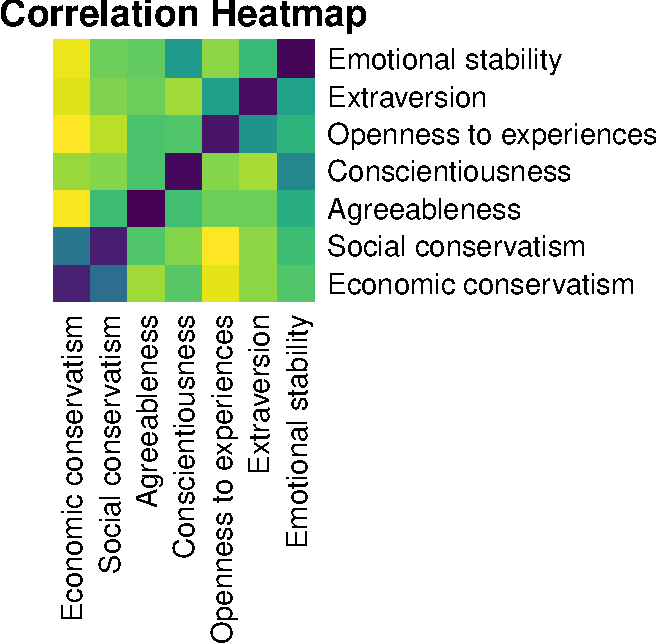
\includegraphics{manuscript_files/figure-latex/correlations-1.pdf}
\caption{}
\end{figure}

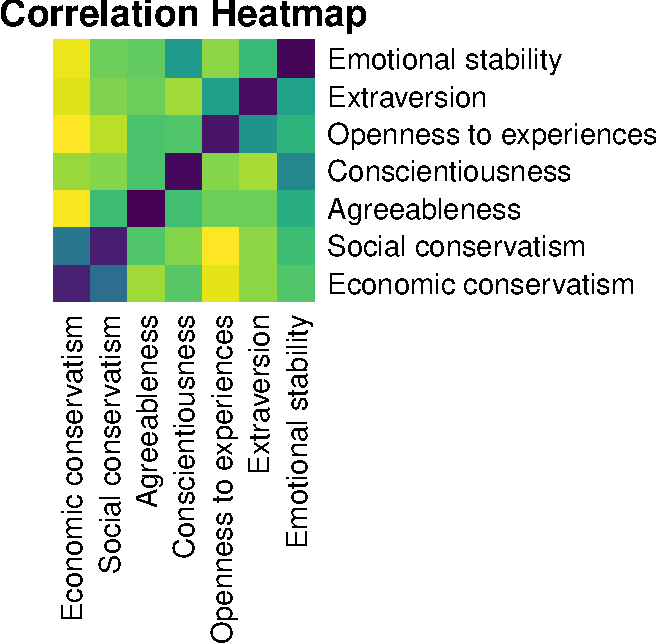
\includegraphics{manuscript_files/figure-latex/figure1-1.pdf}

```

\endgroup


\end{document}
